\begin{figure*}[!t]
\centering
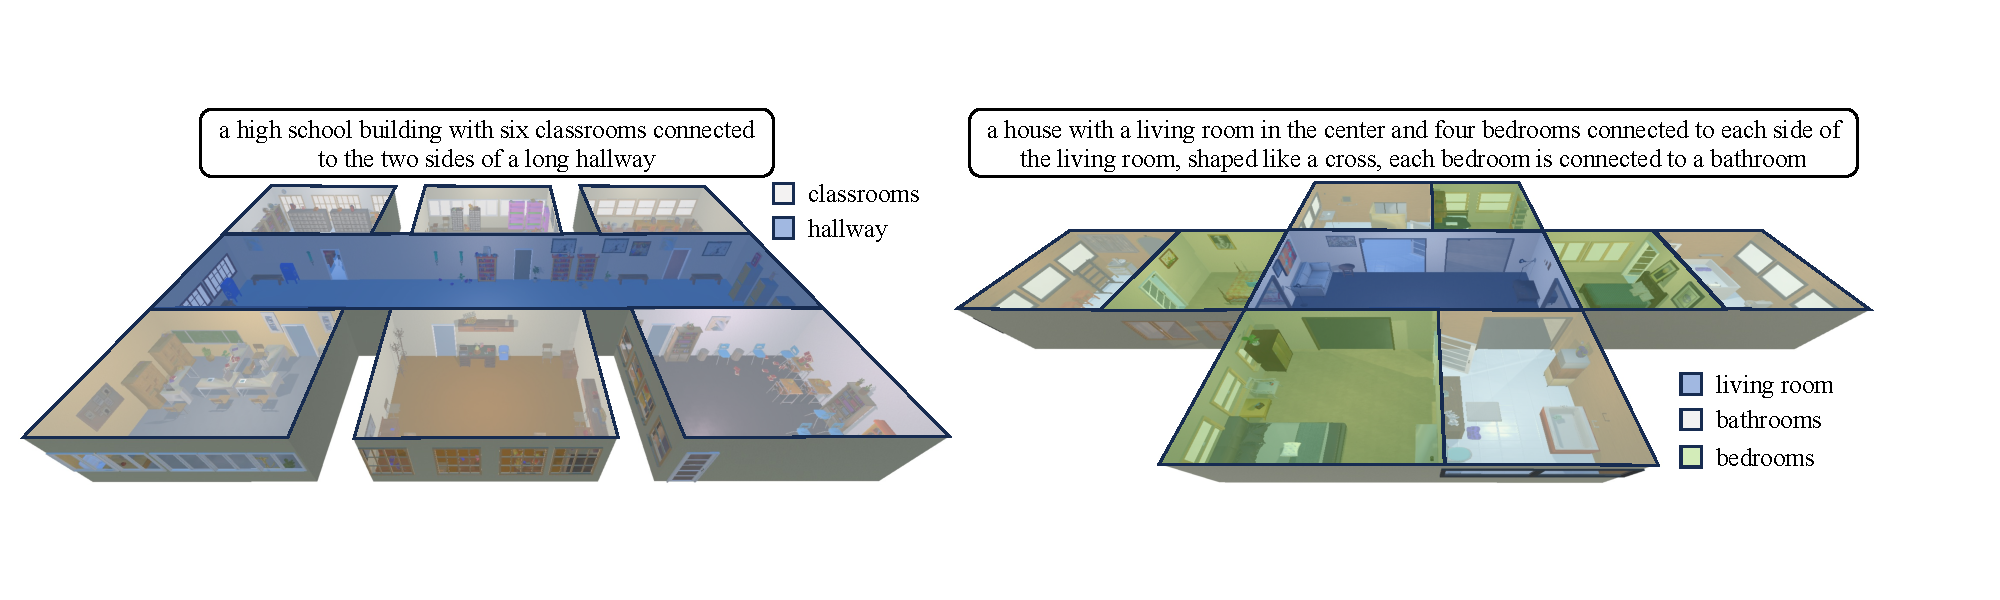
\includegraphics[width=\textwidth]{images/floor_plan_1.pdf}
    \caption{\textbf{Floorplan Customizability.} \holodeck can interpret complicated input and craft reasonable floor plans correspondingly.}
    \label{fig: floor_plan}
    \vspace{-0.2cm}
\end{figure*}

\begin{figure*}[!t]
\centering
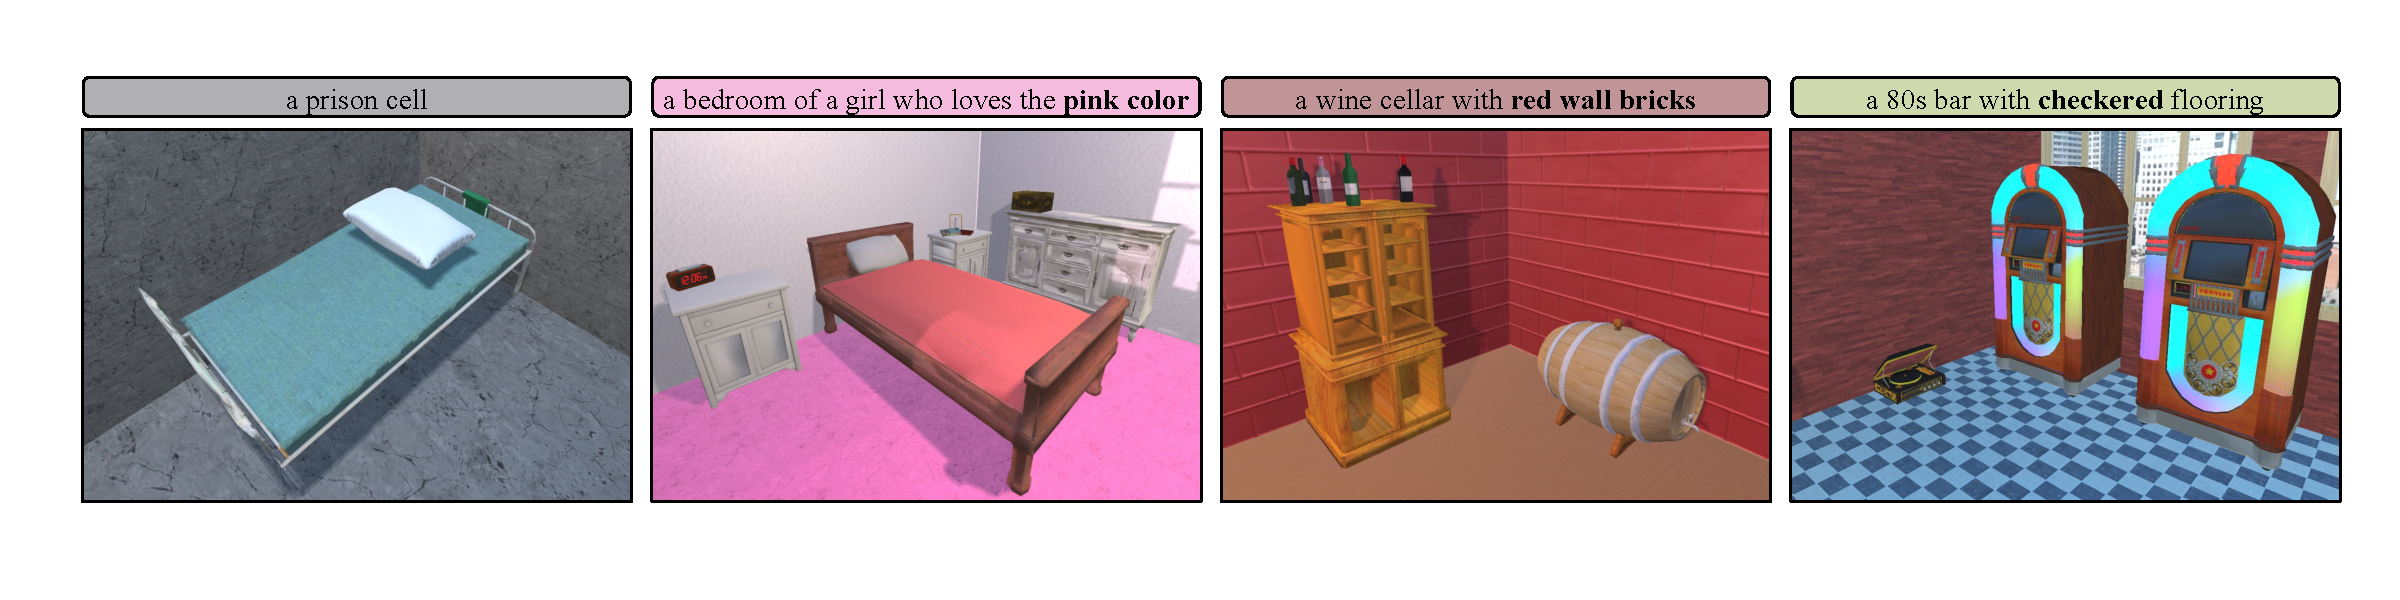
\includegraphics[width=\textwidth]{images/material.pdf}
    \caption{\textbf{Material Customizability.} \holodeck can select appropriate floor and wall materials to make the scenes more realistic.}
    \label{fig: material}
    \vspace{-0.2cm}
\end{figure*}

\begin{figure*}[!t]
\centering
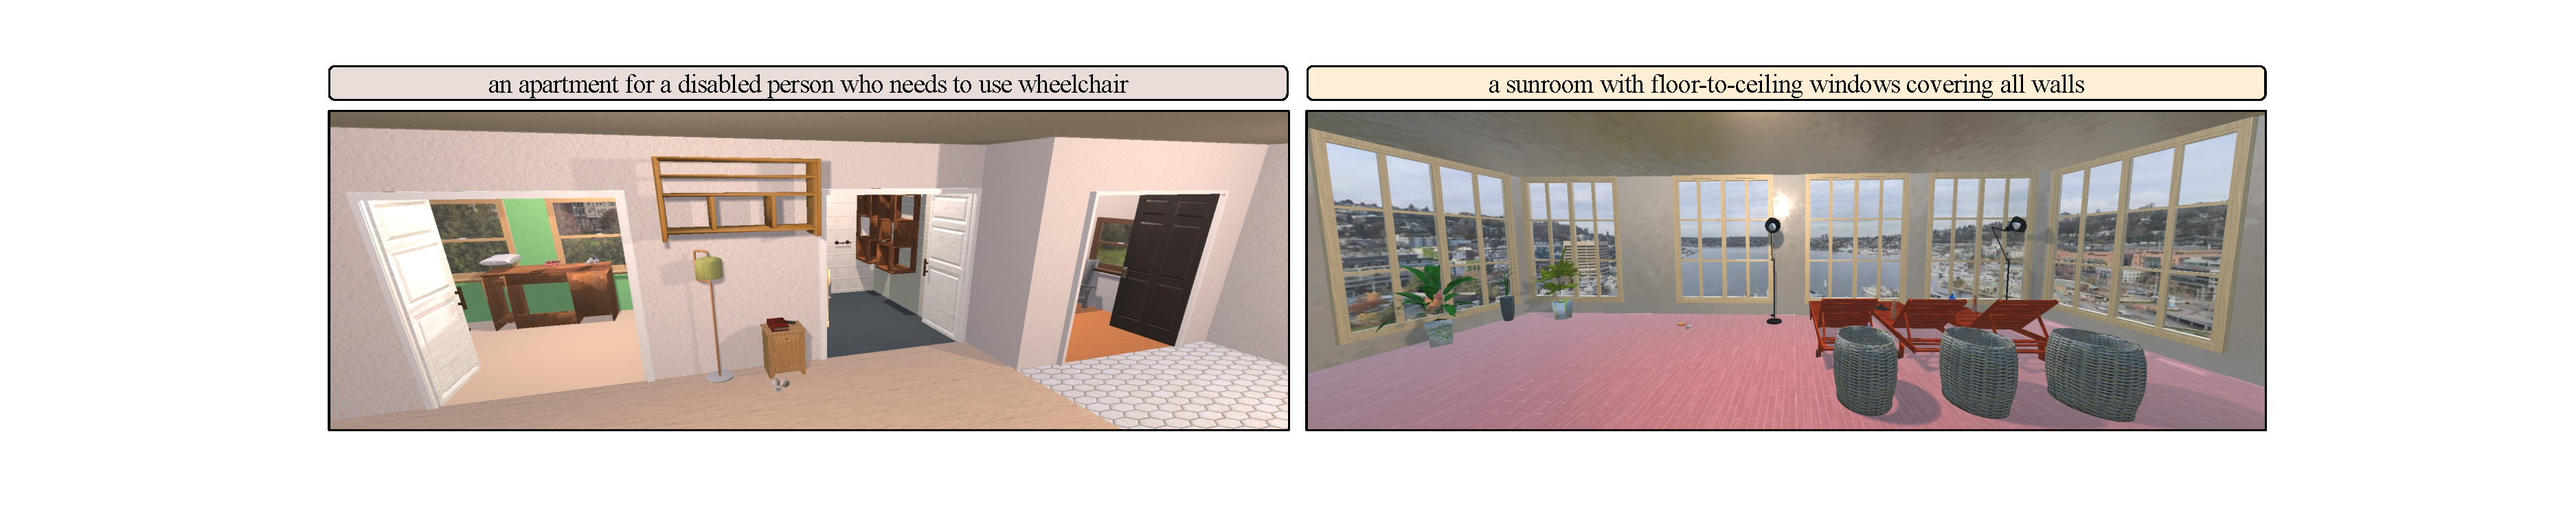
\includegraphics[width=\textwidth]{images/window_door.pdf}
    \caption{\textbf{Door \& window Customizability.} \holodeck can adjust the size, quantity, position, etc., of doors \& windows based on the input.}
    \label{fig: window_door}
    \vspace{-0.35cm}
\end{figure*}
% high level
\holodeck is a promptable system based on AI2-THOR \cite{ai2thor, procthor}, enriched with massive assets from Objaverse~\cite{deitke2023objaverse}, which can produce diverse, customized, and interactive Embodied AI environments with the guidance of large language models.
 % dive into the modules 
 
As shown in Figure \ref{fig: pipeline}, \holodeck employs a systematic approach to scene construction, utilizing a series of specialized modules: (1) the \textit{Floor \& Wall Module} develop floor plans, constructs wall structures and selects appropriate materials for the floors and walls; (2) the \textit{Doorway \& Window Module} integrates doorways and windows into the environment; (3) the \textit{Object Selection Module} retrieves appropriate 3D assets from Objaverse, and (4) the \textit{Constraint-based Layout Design Module} arranges the assets within the scene by utilizing spatial relational constraints to ensure that the layout of objects is realistic.

% These modules process high-level proposals generated by an LLM (GPT-4 \cite{openai2023gpt}) and transform these {prompts/ instructions?} into detailed, numerical specifications for a comprehensive 3D scene. 
%The architecture of \holodeck, depicted in Figure \ref{fig: pipeline}, with each component responsible for different aspects of scene generation. 


In the following sections, we introduce our prompting approach that converts high-level user natural language specifications into a series of language model queries for constructing layouts. 
We then provide a detailed overview of each module shown in Figure~\ref{fig: pipeline} and how they contribute to the final scene. %\textbf{Constraints-based Layout Module}, which searches for designs consistent with language model-derived information. 
Finally, we illustrate how \holodeck leverages Objaverse assets to ensure diversity in scene creation and efficiency for Embodied AI applications. Comprehensive details of \holodeck can be found in the supplement.


% This section begins with an introduction to the \textbf{Prompts} we use that facilitates \holodeck's customizability, followed by a detailed overview of each \textbf{module}. We then highlight our proposed \textbf{Constraints-based Layout Design}, a key feature for efficiently organizing objects within environments. Finally, we show how \holodeck leverages Objaverse Assets to ensure diversity and efficiency in scene creation. Comprehensive details of \holodeck can be found in the supplementary materials.


%This section introduces 
\smallbreak
\noindent \textbf{Overall Prompt Design.} %Prompt engineering offers easy interaction with LLMs through natural language to accomplish tasks without training data.
%One key property of \holodeck is the generation process can be controlled by natural language and thus endow its extensive customizability. 
Each module in Figure~\ref{fig: pipeline} takes information from a language model and converts it to elements included in the final layout.
An LLM prompt is designed for each module with three elements: (1) \textit{Task Description}: outlines the context and goals of the task; (2) \textit{Output Format}: specifies the expected structure and type of outputs and (3) \textit{One-shot Example}: a concrete example to assist the LLM's comprehension of the task. The text within the blue dialog boxes of Figure \ref{fig: pipeline} represents examples of simplified prompts\footnote{The complete prompts (available in the supplementary materials) include additional guidance for LLMs to avoid common errors we observe. For example, by adding a sentence, ``the minimal area per room is 9 m$^2$'', \holodeck can avoid generating overly small rooms.}. LLM's high-level responses to these prompts are post-processed and then used as input arguments for the modules to yield low-level specifications of the scene.%, such as object positions and orientations.

% One key characteristic of \holodeck is its ability to be guided through natural language, providing it with a high degree of customizability. A corresponding prompt is designed for each aforementioned module with three essential elements:(1) \textit{Task Description}, which outlines the context and goals of the task; (2) \textit{Output Format}, detailing the expected structure and type of outputs and (3) \textit{One-shot Example}, offering a tangible example to assist the Large Language Model's (LLM) comprehension of the task. The text in the blue dialog boxes of Figure \ref{fig: pipeline} shows simplified prompt examples. We also include additional instructions to prevent the generation of LLMs from making common mistakes such as impractically small rooms, {add a few more examples}. These instructions include directive sentences such as ``the minimal area per room is 9 m$^2$'', {more examples} (full versions of these prompts are available in section~\ref{appendix: prompt}). The responses generated by the LLM to these prompts are then used as input arguments for the modules, leading to a {detailed/comprehesive?} set of low-level specifications of the scene, which includes the positioning and orientation of objects.

% \smallbreak
% \noindent \textbf{Floor \& Wall Module.} This module designs the floor plans, wall structures, and floor/wall materials. Each room is simplified as a rectangle in \holodeck, which can be defined by a tuple of four representing the corners' coordinates. GPT-4 has a strong spatial ability to provide reasonable dimensions and interconnectivity of the rooms. Figure \ref{fig: floor_plan} shows \holodeck can populate complex, multi-room floor plans that adhere to the prompts, e.g., ``six classrooms connected to the two sides of a hallway'' or ``arrange the rooms to shape like a cross''.
\smallbreak
\noindent The \textbf{Floor \& Wall Module}, illustrated in the first panel of Figure~\ref{fig: pipeline}, is responsible for creating floor plans, constructing wall structures, and selecting materials for floors and walls.
Each room is represented as a rectangle, defined by four tuples that specify the coordinates of its corners.
GPT-4 directly yields the coordinates for placing the rooms and suggests realistic dimensions and connectivity for these rooms.
Figure \ref{fig: floor_plan} illustrates several examples of diverse layouts this module proposes where \holodeck generates prompt-appropriate, intricate, multi-room floor plans. 
%Examples include creating a room layout of ``six classrooms connected to the two sides of a hallway'' or ``arranging rooms to form a cross-like shape.''
\begin{figure*}[!t]
\centering
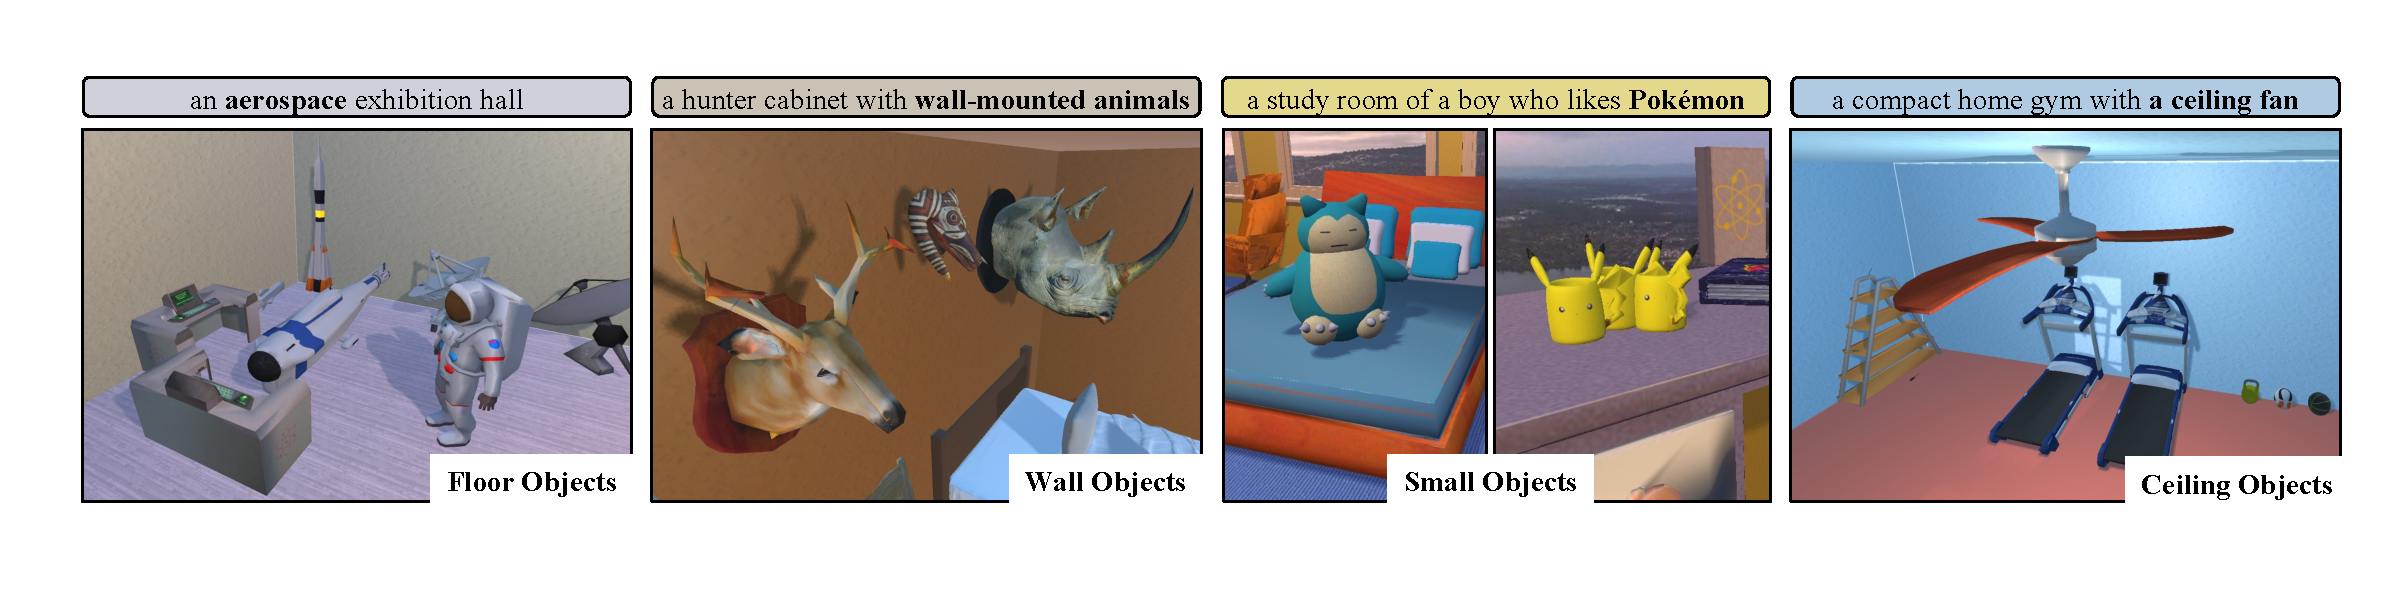
\includegraphics[width=\textwidth]{images/assets.pdf}
    \caption{\textbf{Objects Customizability.} \holodeck can select and place appropriate floor/wall/small/ceiling objects conditioned on the input.}
    \label{fig: asset}
    \vspace{-0.2cm}
\end{figure*}

\begin{figure*}[!t]
\centering
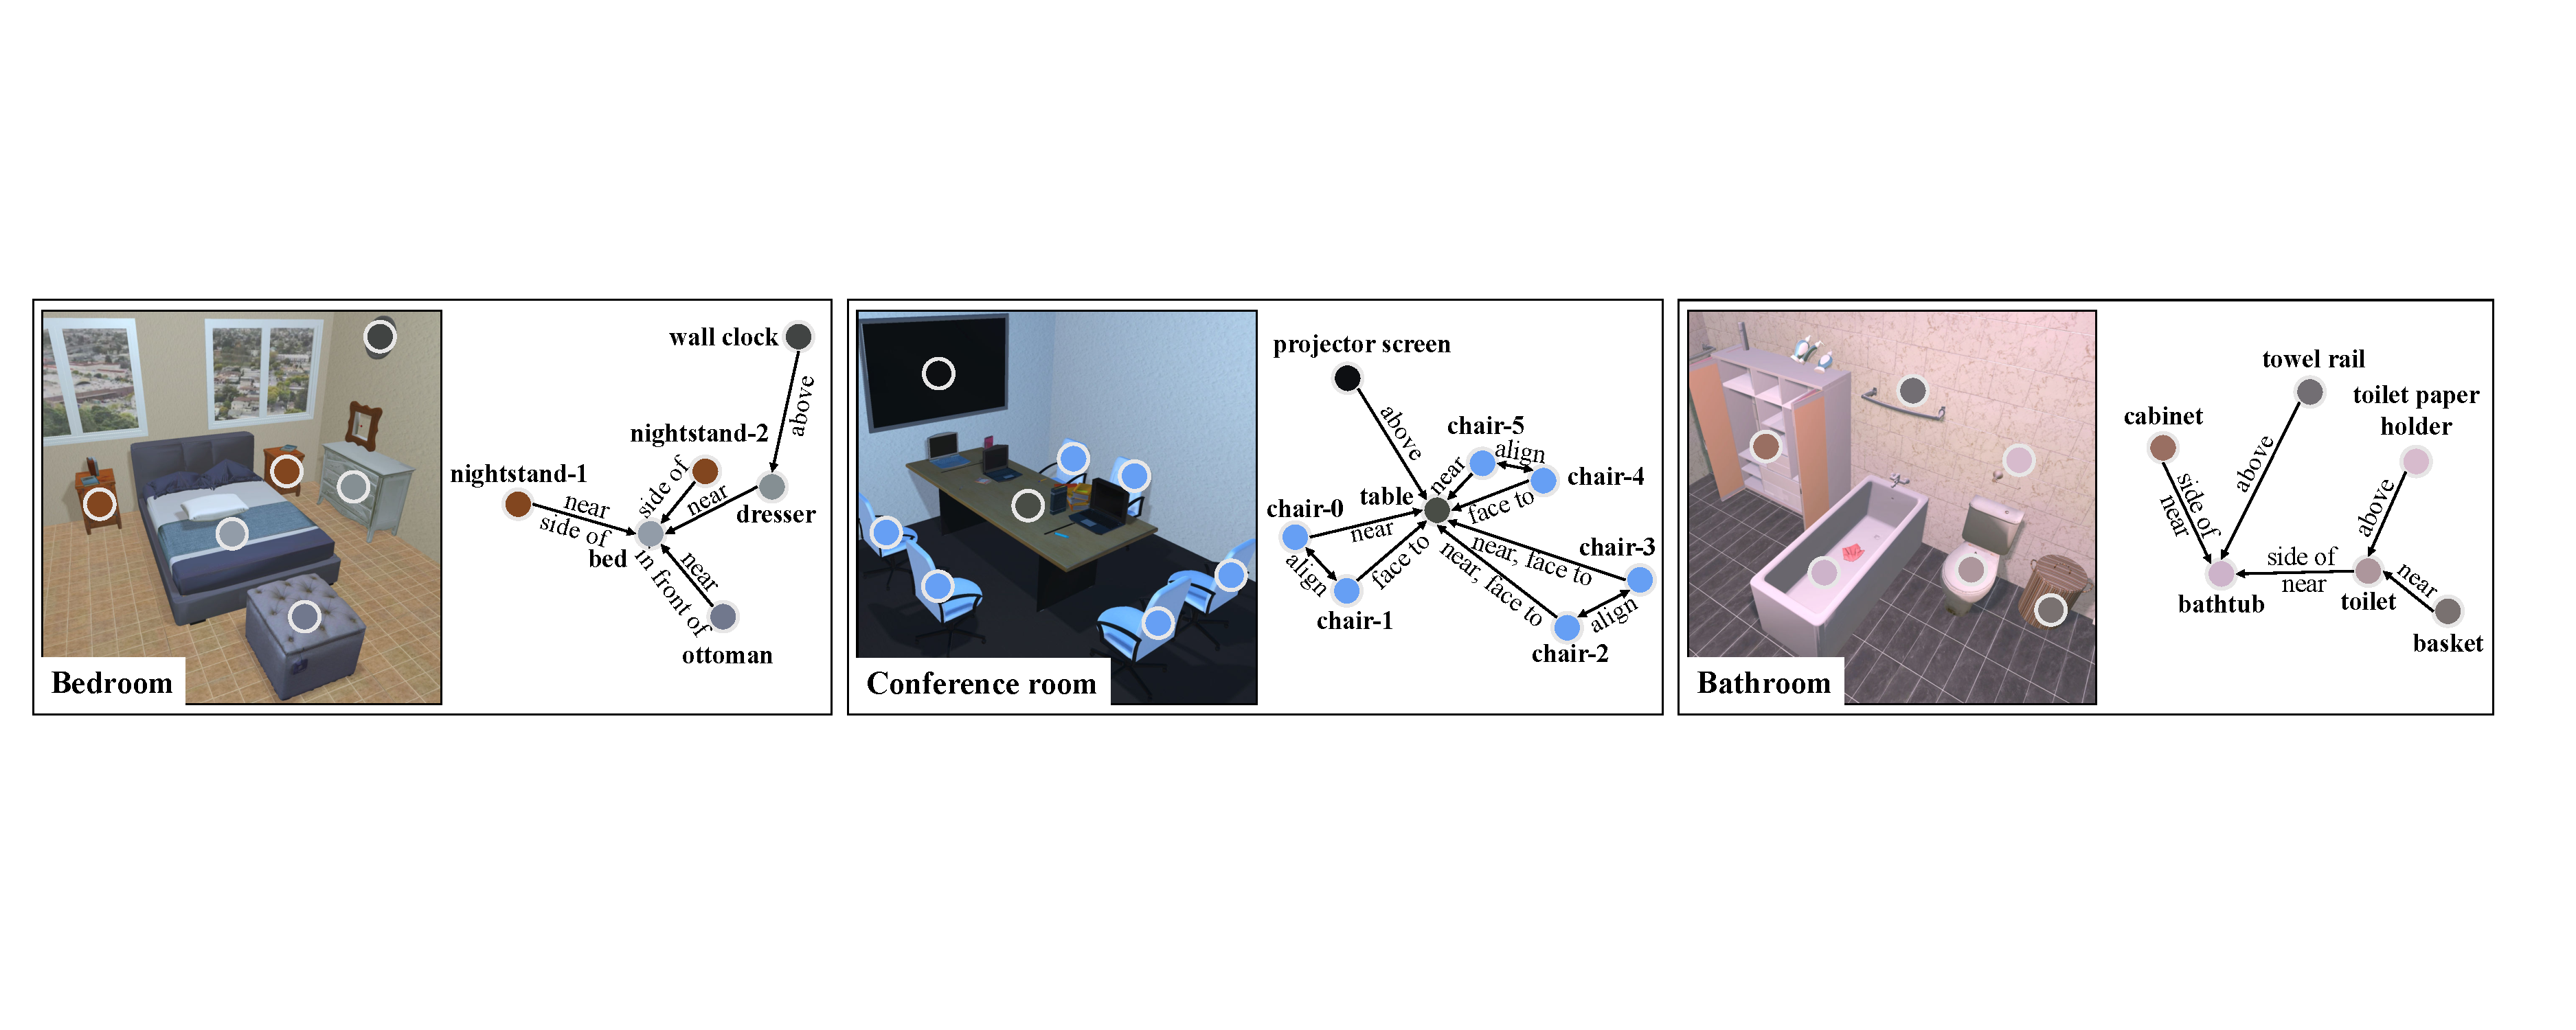
\includegraphics[width=\textwidth]{images/constraints.pdf}
    \caption{Examples of \textbf{Spatial Relational Constraints} generated by LLM and their solutions found by our constraint satisfaction algorithm.}
    \label{fig: constraints}
    \vspace{-0.2cm}
\end{figure*}

\begin{figure*}[!t]
\centering
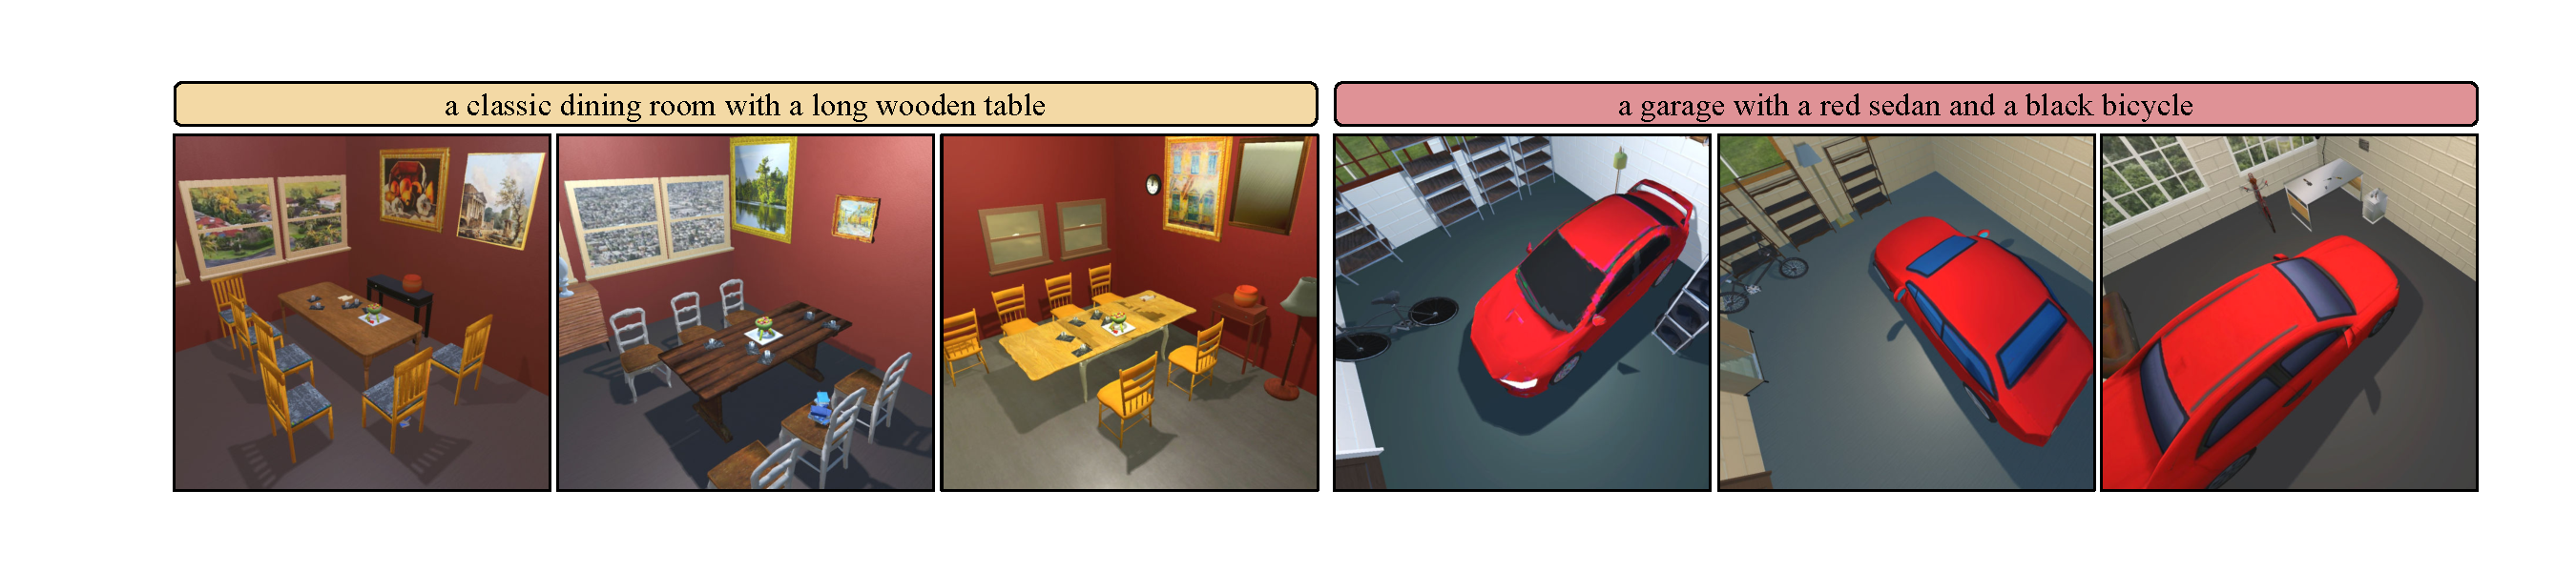
\includegraphics[width=\textwidth]{images/variants.pdf}
    \caption{\textbf{Output Diversity.} \holodeck can generate \textbf{multiple variants} for the same input with different assets and layouts.}
    \label{fig: variants}
    \vspace{-0.5cm}
\end{figure*}
\smallbreak
This module also chooses materials for the floors and walls, which is crucial for enhancing the realism of environments.
\holodeck can match LLM proposals to one of 236 materials, each available in 148 colors, enabling semantic customization of scenes. 
As shown in Figure \ref{fig: material}, \holodeck can generate scenes with suitable materials based on the type of scene, such as opting for concrete walls and floors in a \textit{prison cell} scenario.
Inputs with specific texture requirements are often reflected in the final design, for example, ``pink color", ``red wall bricks," and ``checkered floor".
\smallbreak
\noindent The \textbf{Doorway \& Window Module}, illustrated in the second panel of Figure~\ref{fig: pipeline}, is responsible for proposing room connections and windows. 
Each of these two properties is queried separately from the LLM.
The LLM can propose doorways and windows that match 40 door styles and 21 window types, each of which can be modified by several properties, including size, height, quantity, etc.
%this module allows for detailed customization in quantity and placement to meet specific design requirements. 
For instance, Figure \ref{fig: window_door} shows \holodeck's tailored designs on doors and windows, such as wider doors for ``wheelchair accessibility'' and multiple floor-to-ceiling windows in a ``sunroom'' setting.
\smallbreak
\noindent The \textbf{Object Selection Module}, illustrated in the third panel of Figure~\ref{fig: pipeline}, allows the LLM to propose objects that should be included in the layout.
Leveraging the extensive Objaverse asset collection, \holodeck can fetch and place diverse objects in the scene.
Queries are constructed with LLM-proposed descriptions and dimensions, like ``multi-level cat tower, 60 $\times$ 60 $\times$ 180 (cm)'' to retrieve the optimal asset from Objaverse.
The retrieval function\footnote{We use CLIP \cite{radford2021learning} to measure the visual similarity, Sentence-BERT \cite{reimers-2019-sentence-bert} for the textual similarity, and 3D bounding box sizes for the dimension.} considers visual and textual similarity and dimensions to ensure the assets match the design. Figure \ref{fig: asset} shows the capability of \holodeck to customize diverse objects on the floor, walls, on top of other items, and even on the ceiling.
\smallbreak
\noindent The \textbf{Constraint-based Layout Design Module}, illustrated in the fourth panel of Figure~\ref{fig: pipeline}, generates the positioning and orientation of objects. Previous work \cite{feng2023layoutgpt} shows LLM can directly provide the absolute value of the object's bounding box. However, when attempting to place a diverse lot of assets within environments, this method frequently leads to out-of-boundary errors and object collisions. To address this, instead of letting LLM directly operate on numerical values, we propose a novel constraint-based approach that employs LLM to generate spatial relations between the objects, e.g., ``coffee table, in front of, sofa'', and optimize the layout based on the constraints. Given the probabilistic nature of LLMs, \holodeck can yield multiple valid layouts given the same prompt as shown in Figure \ref{fig: variants}.
%In addition, \holodeck accepts arbitrary text as input, with the scene generation process guided by LLM, which can yield different outputs upon repeated runs. Therefore, \holodeck can produce an unlimited variety of environments. Figure \ref{fig: variants} shows that \holodeck can generate variants of a given design without querying LLM again by altering assets and layouts.
\smallbreak
\noindent \textit{Spatial Relational Constraints.} We predefined ten types of constraints, organized into five categories: (1) Global: \textit{edge}, \textit{middle}; (2) Distance: \textit{near}, \textit{far}; (3) Position: \textit{in front of}, \textit{side of}, \textit{above}, \textit{on top of}; (4) Alignment: \textit{center aligned} and (5) Rotation: \textit{face to}. LLM selects a subset of constraints for each object, forming a scene graph for the room (examples shown in Figure \ref{fig: constraints}). Those constraints are treated softly, allowing for certain violations when finding a layout to satisfy all constraints is not feasible. Besides those soft constraints, we enforce hard constraints to prevent object collisions and ensure that all objects are within the room's boundaries. 
\smallbreak
\noindent \textit{Constraint Satisfaction.} We first reformulate the spatial relational constraints defined above into mathematical conditions (e.g., two objects are center-aligned if they share the same $x$ or $y$ coordinate). To find layouts that satisfy constraints sampled by LLMs, we adopt an optimization algorithm to place objects autoregressively. The algorithm first uses LLM to identify an anchor object and then explores placements for the anchor object. Subsequently, it employs Depth-First-Search (DFS)\footnote{Given the linear nature of constraints, a Mixed Integer Linear Programming (MILP) solver can also be employed. While we assume the DFS solver in our experiments, we analyze the MILP solver in the supplements.} to find valid placements for the remaining objects. A placement is only valid if all the hard constraints are satisfied.
% \footnote{The algorithm will stop if no valid placement is found for an object.}
For example, in Figure \ref{fig: constraints}, \textit{bed} is selected as the anchor object in the \textit{bedroom}, and the \textit{nightstands} are placed subsequently. The algorithm is executed for a fixed time (30 seconds) to get multiple candidate layouts and return the one that satisfies the most total constraints. We verify the effectiveness of our constraint-based layout in Sec \ref{sec: layout ablation}.


% \textbf{\ani{Slightly off heading for this content. When I read Scale, I thought about the size of rooms / environments with many rooms etc. Perhaps you can refer to this as sampling, and then give some details on how you sample, and how this can lead to an exponential generation of envs.}
% }
%\medbreak



\smallbreak
\noindent \textbf{Leveraging Objaverse Assets}, \holodeck is able to support the creation of diverse and customized scenes. 
% Accepting arbitrary text as input and using LLM, \holodeck can produce an unlimited variety of environments.
% \holodeck can yield different outputs upon repeated runs with the same prompt. Figure \ref{fig: variants} shows that \holodeck can generate variants of a given design without querying LLM again by altering assets and layouts.
%A comprehensive and varied asset library is the prerequisite to support the creation of diverse and customized scenes. Leveraging 
We curate a subset of assets suitable for indoor design from \href{https://objaverse.allenai.org/objaverse-1.0/}{Objaverse 1.0}. These assets are further annotated by GPT-4-Vison \cite{openai_2023_gpt4vision} automatically with additional details, including textual descriptions, scale, canonical views, etc.\footnote{GPT-4-Vision can take in multiple images, we prompt it with multi-view screenshots of 3D assets to get the annotations.} Together with the assets from \procthor, our library encompasses 51,464 annotated assets.
% Efficiency
To import Objaverse assets into AI2-THOR for embodied AI applications, we optimize the assets by reducing mesh counts to minimize the loading time in AI2-THOR, generating visibility points and colliders. More details on importing Objaverse assets into AI2-THOR are available in the supplementary materials.



% To summarize, \holodeck provides a flexible way to generate diverse Embodied AI environments through text input.
In the following sections, we will evaluate the quality and utility of the scenes generated by \holodeck.
